% Presentación de 10 minutos (incluye la demostración en vivo del simulador).
% Compilar con: ./docs/compilar_pdf.sh 06_presentacion
\documentclass[aspectratio=169,11pt,xcolor={dvipsnames,table}]{beamer}
\usepackage[utf8]{inputenc}
\usepackage[T1]{fontenc}
\usepackage{lmodern}
\usepackage[spanish,es-nodecimaldot,es-noshorthands,es-tabla]{babel}
\usepackage{amsmath,amssymb}
\usepackage{siunitx}
\sisetup{output-decimal-marker={.},group-digits=false,per-mode=symbol}
\usepackage{booktabs}
\usepackage{tikz}
\usetikzlibrary{arrows.meta,positioning,calc}

\graphicspath{{../../simulacion/graficas/}{figuras/}}
% Archivo generado automáticamente por `generador-axial reporte`. No editar a mano.
\newcommand{\ValGradoIman}{N38}  % Grado comercial del imán
\newcommand{\ValBr}{1.25}  % Remanencia [T]
\newcommand{\ValDiametroIman}{20}  % [mm]
\newcommand{\ValRadioIman}{10.0}  % [mm]
\newcommand{\ValEspesorIman}{5.0}  % [mm]
\newcommand{\ValAreaImanMM}{314.16}  % [mm^2]
\newcommand{\ValPolos}{8}
\newcommand{\ValParesPolos}{4}
\newcommand{\ValPasoPolarGrados}{45.0}  % [grados]
\newcommand{\ValRadioMontaje}{40.0}  % [mm]
\newcommand{\ValBobinas}{8}
\newcommand{\ValEspiras}{180}
\newcommand{\ValEspirasTotales}{1440}
\newcommand{\ValDiametroInteriorBobina}{12.0}  % [mm]
\newcommand{\ValDiametroExteriorBobina}{28.0}  % [mm]
\newcommand{\ValAlturaBobina}{6.0}  % [mm]
\newcommand{\ValEntrehierro}{2.5}  % [mm]
\newcommand{\ValEntrehierroMasAltura}{8.5}  % [mm]
\newcommand{\ValAcoplamiento}{0.85}
\newcommand{\ValCalibreAWG}{26}
\newcommand{\ValDiametroCobre}{0.404}  % [mm]
\newcommand{\ValDiametroEsmaltado}{0.455}  % [mm]
\newcommand{\ValAreaCobreMM}{0.1282}  % [mm^2]
\newcommand{\ValResistividadCobre}{1.72}  % [1e-8 ohm m]
\newcommand{\ValLongitudMediaEspira}{62.83}  % [mm]
\newcommand{\ValLongitudAlambreBobina}{11.31}  % [m]
\newcommand{\ValLongitudAlambreTotal}{90.48}  % [m]
\newcommand{\ValResistenciaBobina}{1.517}  % [ohm]
\newcommand{\ValResistenciaInterna}{12.14}  % [ohm]
\newcommand{\ValVentanaBobinaMM}{48.0}  % [mm^2]
\newcommand{\ValOcupacion}{0.78}
\newcommand{\ValRaizCaraIman}{11.1803}  % sqrt(L^2+R^2) [mm]
\newcommand{\ValTerminoCaraIman}{0.4472}  % L/sqrt(L^2+R^2)
\newcommand{\ValCampoCaraIman}{0.2795}  % [T]
\newcommand{\ValEntrehierroMasEspesor}{7.5}  % g+L [mm]
\newcommand{\ValRaizGL}{12.5000}  % sqrt((g+L)^2+R^2) [mm]
\newcommand{\ValRaizG}{10.3078}  % sqrt(g^2+R^2) [mm]
\newcommand{\ValTerminoUnoG}{0.6000}  % (g+L)/sqrt((g+L)^2+R^2)
\newcommand{\ValTerminoDosG}{0.2425}  % g/sqrt(g^2+R^2)
\newcommand{\ValCampoCaraBobina}{0.2234}  % [T]
\newcommand{\ValEntrehierroAlturaEspesor}{13.5}  % g+h+L [mm]
\newcommand{\ValRaizGHL}{16.8003}  % sqrt((g+h+L)^2+R^2) [mm]
\newcommand{\ValRaizGH}{13.1244}  % sqrt((g+h)^2+R^2) [mm]
\newcommand{\ValPrimitivaEnG}{2.1922}  % F(g) [mm]
\newcommand{\ValPrimitivaEnGH}{3.6759}  % F(g+h) [mm]
\newcommand{\ValDiferenciaPrimitivas}{1.4837}  % F(g+h)-F(g) [mm]
\newcommand{\ValCampoMedioBobina}{0.1545}  % [T]
\newcommand{\ValReduccionPorPromedio}{30.8}  % [%]
\newcommand{\ValFlujoMaximoMicro}{41.270}  % [uWb]
\newcommand{\ValAreaImanM}{3.1416}  % [1e-4 m^2]
\newcommand{\ValCaidaDiodo}{0.30}  % [V]
\newcommand{\ValCaidaPuente}{0.60}  % [V]
\newcommand{\ValCapacitanciaMicro}{220}  % [uF]
\newcommand{\ValTensionNominalCondensador}{50}  % [V]
\newcommand{\ValRpmMaxima}{1200}
\newcommand{\ValTensionDcMaxima}{29.27}  % [V]
\newcommand{\ValMargenCondensador}{41}  % [%]
\newcommand{\ValResistenciaLed}{2200}  % [ohm]
\newcommand{\ValPotenciaNominalResistenciaLed}{0.50}  % [W]
\newcommand{\ValCaidaLed}{2.0}  % [V]
\newcommand{\ValCorrienteLedRefMili}{2.21}  % [mA]
\newcommand{\ValCorrienteLedMaxMili}{12.4}  % [mA]
\newcommand{\ValCorrienteLedLimiteMili}{20}  % [mA]
\newcommand{\ValPotenciaResistenciaLedMax}{0.338}  % [W]
\newcommand{\ValRizadoRef}{251.4}  % [mV]
\newcommand{\ValRpmReferencia}{300}
\newcommand{\ValOmegaMecanicaRef}{31.416}  % [rad/s]
\newcommand{\ValFrecuenciaRef}{20.00}  % [Hz]
\newcommand{\ValPeriodoRefMs}{50.00}  % [ms]
\newcommand{\ValOmegaElectricaRef}{125.66}  % [rad/s]
\newcommand{\ValTensionPicoRef}{7.47}  % [V]
\newcommand{\ValTensionRmsRef}{5.28}  % [V]
\newcommand{\ValTensionDcRef}{6.87}  % [V]
\newcommand{\ValTensionPicoPorBobinaRef}{0.933}  % [V]
\newcommand{\ValRpmCarga}{400}
\newcommand{\ValOmegaMecanicaCarga}{41.89}  % [rad/s]
\newcommand{\ValTensionPicoCarga}{9.96}  % [V]
\newcommand{\ValTensionRmsCarga}{7.04}  % [V]
\newcommand{\ValCorrienteCarga}{0.290}  % [A]
\newcommand{\ValTensionEnCarga}{3.52}  % [V]
\newcommand{\ValPotenciaCarga}{1.021}  % [W]
\newcommand{\ValPotenciaPerdidas}{1.021}  % [W]
\newcommand{\ValPotenciaMecanica}{2.042}  % [W]
\newcommand{\ValParResistenteMili}{48.7}  % [mN m]
\newcommand{\ValEficiencia}{50}  % [%]
\newcommand{\ValBateriaTension}{12}  % [V]
\newcommand{\ValBateriaCapacidad}{7}  % [Ah]
\newcommand{\ValBateriaEnergia}{84}  % [Wh]
\newcommand{\ValBateriaResistencia}{0.05}  % [ohm]
\newcommand{\ValBateriaVacia}{11.8}  % E_oc con SoC = 0 [V]
\newcommand{\ValBateriaLlena}{12.8}  % E_oc con SoC = 1 [V]
\newcommand{\ValBateriaPendiente}{1.0}  % [V]
\newcommand{\ValSocInicial}{50}  % [%]
\newcommand{\ValSocCorte}{20}  % [%]
\newcommand{\ValSocReconexion}{25}  % [%]
\newcommand{\ValTensionOcRef}{12.30}  % [V]
\newcommand{\ValEnergiaUtilRef}{25.2}  % [Wh]
\newcommand{\ValControladorEficiencia}{90}  % [%]
\newcommand{\ValControladorArranque}{3.5}  % [V]
\newcommand{\ValControladorCorrienteMax}{3.0}  % [A]
\newcommand{\ValControladorAbsorcion}{14.4}  % [V]
\newcommand{\ValRpmMicrored}{600}
\newcommand{\ValFemRmsMicrored}{10.56}  % [V]
\newcommand{\ValTensionDcMicrored}{14.34}  % [V]
\newcommand{\ValPotenciaExtraibleMicrored}{2.297}  % [W]
\newcommand{\ValPotenciaHaciaBateria}{2.067}  % [W]
\newcommand{\ValCorrienteCargaMicroredMili}{168}  % [mA]
\newcommand{\ValPotenciaMecanicaMicrored}{4.59}  % [W]
\newcommand{\ValParMicroredMili}{73.1}  % [mN m]
\newcommand{\ValHorasRecarga}{20.8}  % [h]
\newcommand{\ValInversorTension}{110}  % [V]
\newcommand{\ValInversorPico}{155.6}  % [V]
\newcommand{\ValInversorTensionAlta}{220}  % [V]
\newcommand{\ValInversorPicoAlto}{311.1}  % [V]
\newcommand{\ValInversorFrecuencia}{60}  % [Hz]
\newcommand{\ValInversorNominal}{150}  % [W]
\newcommand{\ValInversorEficiencia}{90}  % [%]
\newcommand{\ValRelacionEspiras}{13.0}  % V_pico,AC / V_bat
\newcommand{\ValPotenciaCargaAc}{15}  % [W]
\newcommand{\ValCorrienteAcMili}{136}  % [mA]
\newcommand{\ValPotenciaEntradaInversor}{16.67}  % [W]
\newcommand{\ValCorrienteInversorBateria}{1.36}  % [A]
\newcommand{\ValPotenciaNetaBateria}{-14.60}  % [W]
\newcommand{\ValAutonomiaHoras}{1.73}  % [h]
\newcommand{\ValAutonomiaParadoHoras}{1.51}  % [h]
\newcommand{\ValRpmEquilibrio}{1704}
\newcommand{\ValPotenciaCargaReducida}{5}  % [W]
\newcommand{\ValRpmEquilibrioReducida}{984}
\newcommand{\ValInerciaRotor}{2.415}  % [1e-4 kg m^2]
\newcommand{\ValInductanciaBobinaMili}{0.528}  % [mH]
\newcommand{\ValInductanciaTotalMili}{4.22}  % [mH]
\newcommand{\ValFlujoMaximoReal}{0.827}  % phi_max normalizado
\newcommand{\ValPicoDerivadaFlujo}{0.746}
\newcommand{\ValRmsDerivadaFlujo}{0.559}
\newcommand{\ValFactorCresta}{1.335}
\newcommand{\ValFactorMedia}{0.706}
\newcommand{\ValRelacionFemRealIdeal}{0.930}
\newcommand{\ValPuntosRadiales}{32}
\newcommand{\ValMuestrasPerfil}{256}
\newcommand{\ValPasoIntegracionMili}{5}  % [ms]
\newcommand{\ValParCoulombMili}{3.0}  % [mN m]
\newcommand{\ValCoefViscosoMicro}{15.0}  % [uN m s]
\newcommand{\ValCoefVentilacionNano}{15.0}  % [nN m s^2]
\newcommand{\ValParMaximoMotriz}{0.30}  % [N m]
\newcommand{\ValVelocidadVacioMotriz}{1500}  % [RPM]
\newcommand{\ValParImpulso}{0.08}  % [N m]
\newcommand{\ValDuracionImpulso}{0.5}  % [s]
\newcommand{\ValCapacidadTermica}{100}  % [J/K]
\newcommand{\ValConveccionNatural}{8}  % [W/m^2K]
\newcommand{\ValConveccionForzada}{0.15}  % [W/m^2K por rad/s]
\newcommand{\ValCoefCobre}{0.393}  % [%/K]
\newcommand{\ValCoefRemanencia}{-0.12}  % [%/K]
\newcommand{\ValTemperaturaMaximaPla}{55}  % [C]
\newcommand{\ValBateriaRCero}{25}  % [mohm]
\newcommand{\ValBateriaRPolarizacion}{30}  % [mohm]
\newcommand{\ValBateriaTau}{30}  % [s]
\newcommand{\ValBateriaPeukert}{1.12}
\newcommand{\ValBateriaEtaCoulomb}{95}  % [%]
\newcommand{\ValBateriaEtaLlena}{60}  % [%]
\newcommand{\ValBateriaSocGas}{85}  % [%]
\newcommand{\ValBateriaAutodescarga}{3}  % [%/mes]
\newcommand{\ValBateriaSocFlotacion}{99.5}  % [%]
\newcommand{\ValBateriaFactorGas}{1500}
\newcommand{\ValBateriaPendienteGas}{50}
\newcommand{\ValControladorFlotacion}{13.8}  % [V]
\newcommand{\ValConsumoControladorMili}{8}  % [mA]
\newcommand{\ValInversorVacio}{3.6}  % [W]
\newcommand{\ValInversorCoefCuadratico}{5.81}  % [1e-4 1/W]
\newcommand{\ValInversorCorte}{10.8}  % [V]
\newcommand{\ValInversorReconexion}{12.3}  % [V]
\newcommand{\ValParReferencia}{0.07}  % [N m]
\newcommand{\ValRpmRegimenRef}{483}
\newcommand{\ValPotenciaEjeRef}{2.40}  % [W]
\newcommand{\ValPotenciaElectromagneticaRef}{2.21}  % [W]
\newcommand{\ValPerdidasCobreRef}{0.986}  % [W]
\newcommand{\ValPerdidasRozamientoRef}{0.192}  % [W]
\newcommand{\ValPerdidasFoucaultMili}{1.65}  % [mW]
\newcommand{\ValPotenciaBateriaRef}{0.96}  % [W]
\newcommand{\ValEficienciaRef}{40}  % [%]
\newcommand{\ValTensionDcRefReal}{3.50}  % [V]
\newcommand{\ValCorrienteGeneradorRef}{0.281}  % [A]
\newcommand{\ValTemperaturaRegimenRef}{27.8}  % [C]
\newcommand{\ValRpmConCargaRef}{483}
\newcommand{\ValPotenciaEntradaInversorRef}{18.7}  % [W]
\newcommand{\ValCorrienteNetaConCarga}{-1.48}  % [A]
\newcommand{\ValRpmParMaximo}{1002}
\newcommand{\ValPotenciaBateriaParMaximo}{4.35}  % [W]
\newcommand{\ValRizadoBajo}{18.8}  % [V] con 220 uF
\newcommand{\ValRizadoAlto}{0.88}  % [V] con 4700 uF
\newcommand{\ValRpmPicoImpulso}{505}
\newcommand{\ValTiempoParadaImpulso}{2.7}  % [s]
\newcommand{\ValHorasHastaAbsorcion}{4.0}  % [h]
\newcommand{\ValHorasHastaFlotacion}{8.2}  % [h]
\newcommand{\ValCorrienteFlotacionMili}{21}  % [mA]


% ---------------------------------------------------------------- estilo
\definecolor{Azul}{HTML}{0D47A1}
\definecolor{Cian}{HTML}{00838F}
\definecolor{Naranja}{HTML}{E65100}
\definecolor{Rojo}{HTML}{C62828}
\definecolor{Verde}{HTML}{2E7D32}
\definecolor{Gris}{HTML}{455A64}

\usefonttheme{professionalfonts}
\setbeamercolor{frametitle}{fg=Azul}
\setbeamerfont{frametitle}{series=\bfseries,size=\Large}
\setbeamercolor{structure}{fg=Azul}
\setbeamercolor{block title}{bg=Azul,fg=white}
\setbeamercolor{block body}{bg=Azul!6}
\setbeamercolor{block title alerted}{bg=Naranja,fg=white}
\setbeamercolor{block body alerted}{bg=Naranja!7}
\setbeamercolor{block title example}{bg=Verde,fg=white}
\setbeamercolor{block body example}{bg=Verde!7}
\setbeamertemplate{navigation symbols}{}
\setbeamertemplate{itemize items}[circle]
\setbeamertemplate{blocks}[rounded]
\setbeamertemplate{footline}{%
  \leavevmode\hbox to\paperwidth{%
    \hspace{1em}{\color{Gris}\tiny Generador de flujo axial con imanes NdFeB}\hfill
    {\color{Gris}\tiny\insertframenumber/\inserttotalframenumber}\hspace{1em}}%
  \vspace{0.6em}}

\newcommand{\dato}[2]{{\small\color{Gris}#1}\\[-1pt]{\Large\bfseries\color{Azul}#2}}

\title{Generador de flujo axial con imanes NdFeB}
\subtitle{Del electromagnetismo de Sadiku a una micro-red simulada en tiempo real}
\date{}

\begin{document}

% ================================================================ 1. Portada  (0:15)
\begin{frame}[plain]
  \begin{tikzpicture}[remember picture,overlay]
    \fill[Azul] (current page.north west) rectangle ([yshift=-4.4cm]current page.north east);
    \node[anchor=north west,text=white,font=\sffamily\bfseries\LARGE,text width=10cm,align=left]
      at ([xshift=1cm,yshift=-1.2cm]current page.north west) {\inserttitle};
    \node[anchor=north west,text=white!85!Azul,font=\sffamily\normalsize,text width=10cm,align=left]
      at ([xshift=1cm,yshift=-2.9cm]current page.north west) {\insertsubtitle};
    \begin{scope}[shift={([xshift=-2.6cm,yshift=-2.2cm]current page.north east)},scale=0.5]
      \foreach \i in {0,...,7} {
        \pgfmathsetmacro{\ang}{45*\i}
        \ifodd\i \def\col{Azul!40}\def\pol{S}\else \def\col{Rojo!80}\def\pol{N}\fi
        \fill[\col] (\ang:2.2) circle (0.55);
        \node[white,font=\bfseries\small] at (\ang:2.2) {\pol};
      }
      \draw[white,line width=1pt] (0,0) circle (3.0);
      \fill[white!70] (0,0) circle (0.35);
    \end{scope}
  \end{tikzpicture}
  \vspace{4.2cm}
  \begin{columns}[T]
    \column{0.5\textwidth}
      \small Teoría Electromagnética\\[2pt]
      \color{Gris}\footnotesize Basado en M.\,N.\,O. Sadiku, \emph{Elementos de Electromagnetismo}, cap.~7--9
    \column{0.42\textwidth}
      \footnotesize\color{Gris}
      Modelo en Python \(\cdot\) Visualizador 3D en Three.js\\
      Piezas imprimibles en 3D \(\cdot\) 5 documentos técnicos
  \end{columns}
\end{frame}

% ================================================================ 2. Sistema  (0:45)
\begin{frame}{¿Qué construimos?}
  \centering
  \begin{tikzpicture}[
      caja/.style={draw=Azul,fill=Azul!6,rounded corners=3pt,minimum height=1.05cm,
                   text width=1.75cm,align=center,font=\scriptsize},
      flecha/.style={-{Stealth[length=2.2mm]},thick,Gris},
      node distance=0.42cm]
    \node[caja,draw=Naranja,fill=Naranja!8] (mano) {Par motriz\\mano / motor};
    \node[caja,right=of mano] (rotor) {Rotor\\\ValPolos{} imanes \ValGradoIman};
    \node[caja,right=of rotor] (bob) {\ValBobinas{} bobinas\\sin núcleo};
    \node[caja,right=of bob] (puente) {Puente\\rectificador};
    \node[caja,right=of puente] (mppt) {Controlador\\MPPT};
    \node[caja,right=of mppt,draw=Verde,fill=Verde!8] (bat) {Batería\\\SI{12}{V} / \SI{7}{Ah}};
    \node[caja,below=0.9cm of bat] (inv) {Inversor\\\SI{110}{}/\SI{220}{V} \SI{60}{Hz}};
    \node[caja,left=of inv,draw=Naranja,fill=Naranja!8] (foco) {Bombillo\\carga AC};
    \draw[flecha] (mano) -- (rotor);
    \draw[flecha] (rotor) -- node[above,font=\tiny]{\(\Phi(t)\)} (bob);
    \draw[flecha] (bob) -- node[above,font=\tiny]{AC} (puente);
    \draw[flecha] (puente) -- node[above,font=\tiny]{DC} (mppt);
    \draw[flecha] (mppt) -- (bat);
    \draw[flecha] (bat) -- (inv);
    \draw[flecha] (inv) -- (foco);
    \draw[flecha,Rojo,dashed] (bob.south) -- ++(0,-0.5) -- node[below,font=\tiny,text=Rojo]
      {par de Lenz: frena el rotor} ([yshift=-0.5cm]rotor.south) -- (rotor.south);
  \end{tikzpicture}

  \vspace{0.5cm}
  \begin{columns}[T]
    \column{0.31\textwidth}
      \begin{block}{Objetivo}\small
        Convertir energía mecánica en eléctrica aplicando la ley de Faraday.
      \end{block}
    \column{0.31\textwidth}
      \begin{block}{Diseño}\small
        Flujo axial, bobinas sin hierro y piezas impresas en PLA.
      \end{block}
    \column{0.31\textwidth}
      \begin{block}{Simulación}\small
        Física completa del sistema, idéntica en Python y en el navegador.
      \end{block}
  \end{columns}
\end{frame}

% ================================================================ 3. Física  (0:50)
\begin{frame}{La física: campo, flujo, Faraday y Lenz}
  \begin{columns}[c]
    \column{0.52\textwidth}
      \small
      \textbf{Campo en el eje de un imán cilíndrico}
      \[
        B_z(z)=\frac{B_r}{2}\left[\frac{z+L}{\sqrt{(z+L)^2+R^2}}-\frac{z}{\sqrt{z^2+R^2}}\right]
      \]
      \textbf{Ley de Faraday} (\(N_t=\ValEspirasTotales\) espiras en serie)
      \[
        \mathcal{E}(t)=-N_t\,\frac{\mathrm{d}\Phi}{\mathrm{d}t}
        \qquad
        f_e=\frac{p}{2}\,\frac{n}{60}
      \]
      \textbf{Ley de Lenz}: la corriente se opone al cambio de flujo
      \[
        \tau_{\text{Lenz}}=\frac{P_{\text{em}}}{\omega_m}
      \]
    \column{0.44\textwidth}
      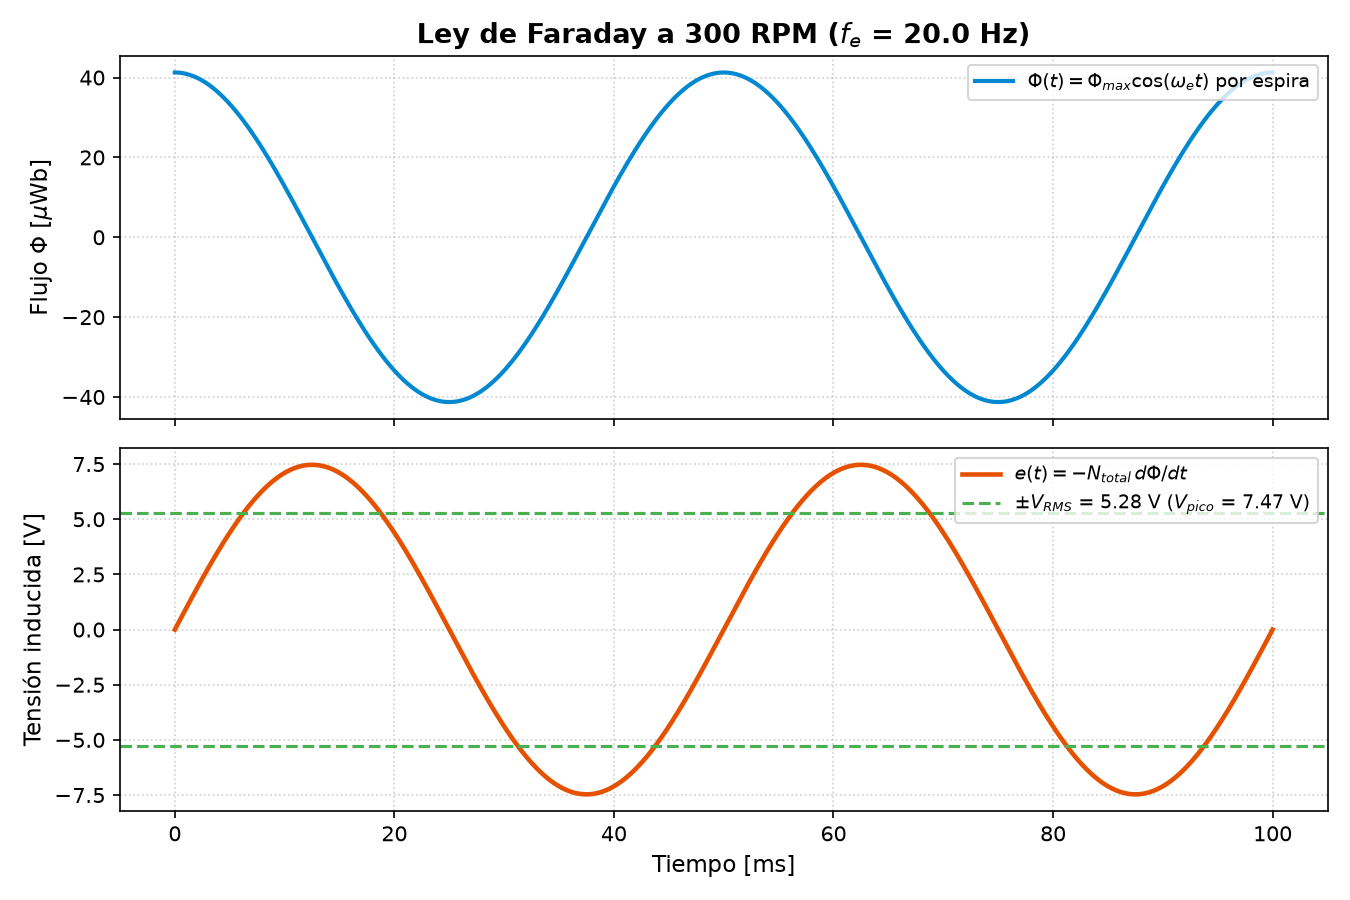
\includegraphics[width=\linewidth]{02_flujo_y_voltaje_inducido_faraday.png}
      \vspace{2pt}
      \begin{center}\footnotesize
        \begin{tabular}{@{}ll@{}}
          \(B\) en la cara del imán & \SI{\ValCampoCaraIman}{T}\\
          \(B\) medio en la bobina & \SI{\ValCampoMedioBobina}{T}\\
          Flujo máximo por espira & \SI{\ValFlujoMaximoMicro}{\micro Wb}
        \end{tabular}
      \end{center}
  \end{columns}
\end{frame}

% ================================================================ 4. Diseño  (0:40)
\begin{frame}{El diseño del generador}
  \begin{columns}[c]
    \column{0.42\textwidth}
      \footnotesize
      \begin{tabular}{@{}lr@{}}
        \toprule
        Imanes & \ValPolos{} \(\times\) \SI{\ValDiametroIman}{}\(\times\)\SI{\ValEspesorIman}{mm}\\
        Remanencia \(B_r\) & \SI{\ValBr}{T}\\
        Bobinas & \ValBobinas{} \(\times\) \ValEspiras{} espiras\\
        Alambre & AWG \ValCalibreAWG{}, \SI{\ValLongitudAlambreTotal}{m}\\
        Entrehierro & \SI{\ValEntrehierro}{mm}\\
        Resistencia interna & \SI{\ValResistenciaInterna}{\ohm}\\
        Inductancia (Wheeler) & \SI{\ValInductanciaTotalMili}{mH}\\
        Inercia del rotor & \SI{\ValInerciaRotor e-4}{kg.m^2}\\
        \bottomrule
      \end{tabular}

      \vspace{8pt}
      \begin{exampleblock}{A \ValRpmReferencia{} RPM}\footnotesize
        \(f_e=\SI{\ValFrecuenciaRef}{Hz}\), \(V_{\text{pico}}=\SI{\ValTensionPicoRef}{V}\),
        \(V_{\text{rms}}=\SI{\ValTensionRmsRef}{V}\)
      \end{exampleblock}
    \column{0.54\textwidth}
      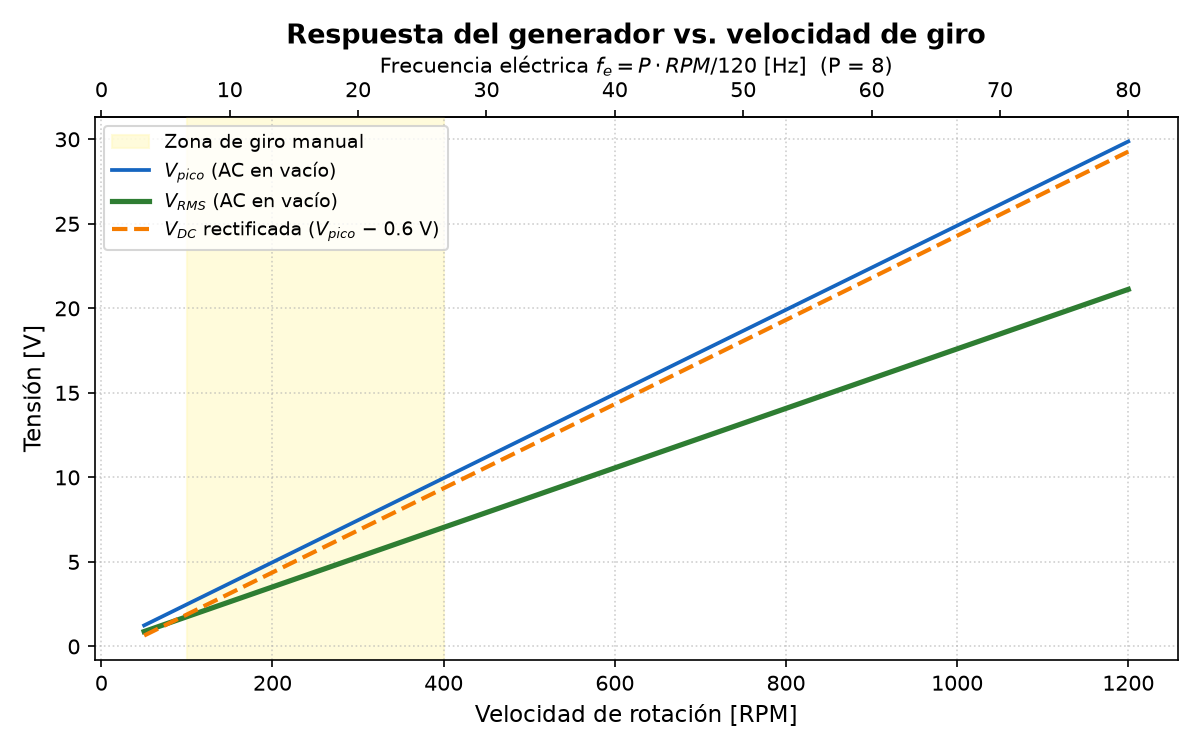
\includegraphics[width=\linewidth]{03_voltaje_rms_vs_rpm.png}
      \\[-2pt]{\scriptsize\color{Gris} La tensión crece linealmente con la velocidad: \(\mathcal{E}\propto\omega\).}
  \end{columns}
\end{frame}

% ================================================================ 5. Modelo realista  (0:50)
\begin{frame}{Del modelo ideal al modelo realista}
  \begin{columns}[c]
    \column{0.5\textwidth}
      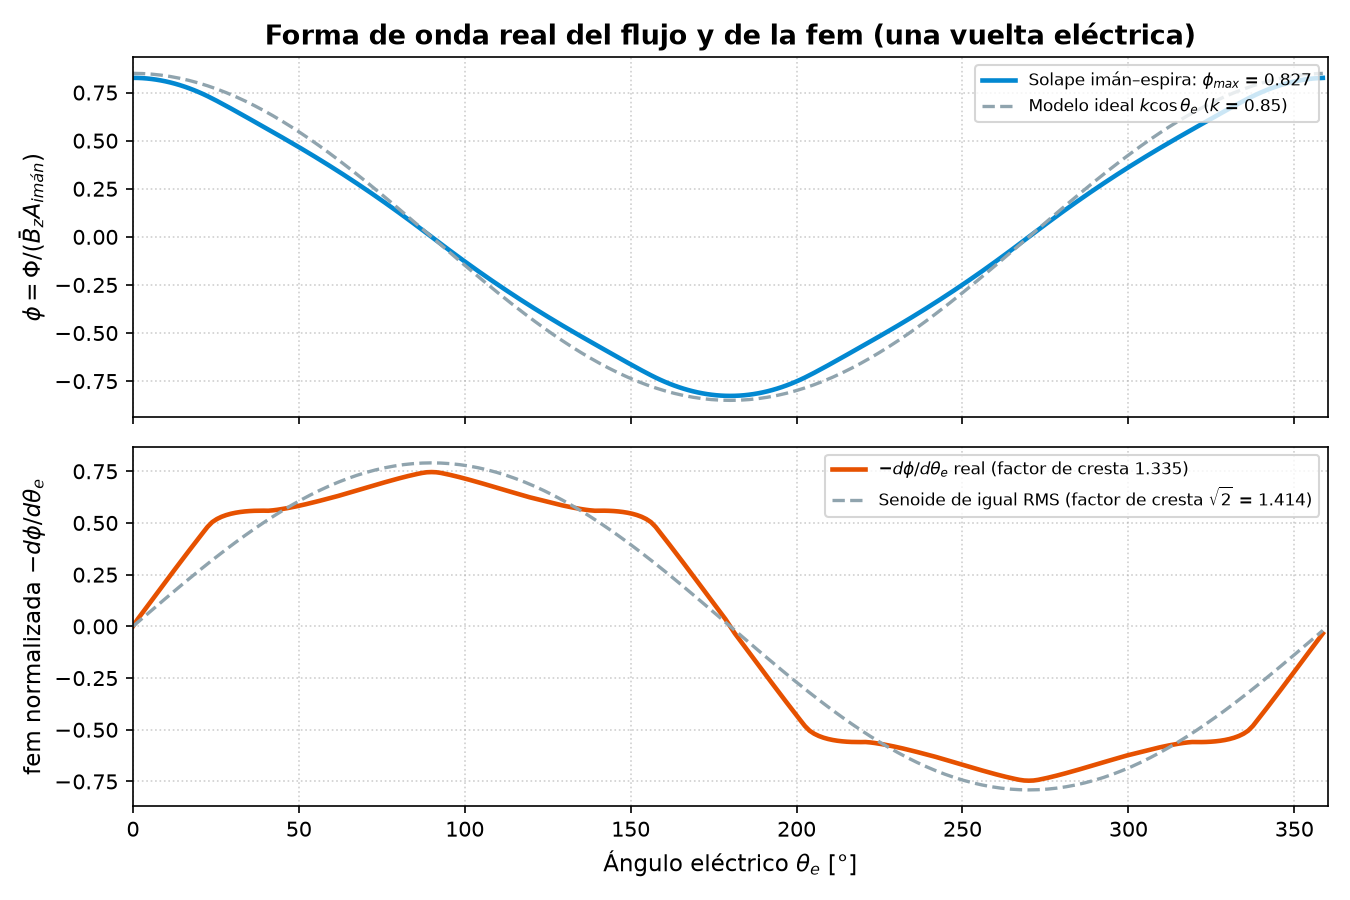
\includegraphics[width=\linewidth]{09_onda_real_vs_senoidal.png}
    \column{0.47\textwidth}
      \small
      \begin{itemize}
        \item \textbf{Onda real}: solape imán--espira; no es senoidal (factor de cresta \ValFactorCresta).
        \item \textbf{Rotor}: \(J\,\dot\omega=\tau_m-\tau_{\text{Lenz}}-\tau_{\text{fricción}}\).
        \item \textbf{Electrónica}: MPPT desde \SI{\ValControladorArranque}{V}, absorción \SI{\ValControladorAbsorcion}{V},
              flotación \SI{\ValControladorFlotacion}{V}, máx.\ \SI{\ValControladorCorrienteMax}{A}.
        \item \textbf{Batería plomo-ácido}: Thevenin, Peukert y gasificación.
        \item \textbf{Inversor}: \SI{\ValInversorVacio}{W} en vacío; corte a \SI{\ValInversorCorte}{V}, reconexión a \SI{\ValInversorReconexion}{V}.
        \item \textbf{Térmico}: \(R_{\text{Cu}}\) sube y \(B_r\) baja con la temperatura.
      \end{itemize}
  \end{columns}
\end{frame}

% ================================================================ 6. Micro-red  (0:40)
\begin{frame}{Dinámica y carga de la batería}
  \begin{columns}[T]
    \column{0.49\textwidth}
      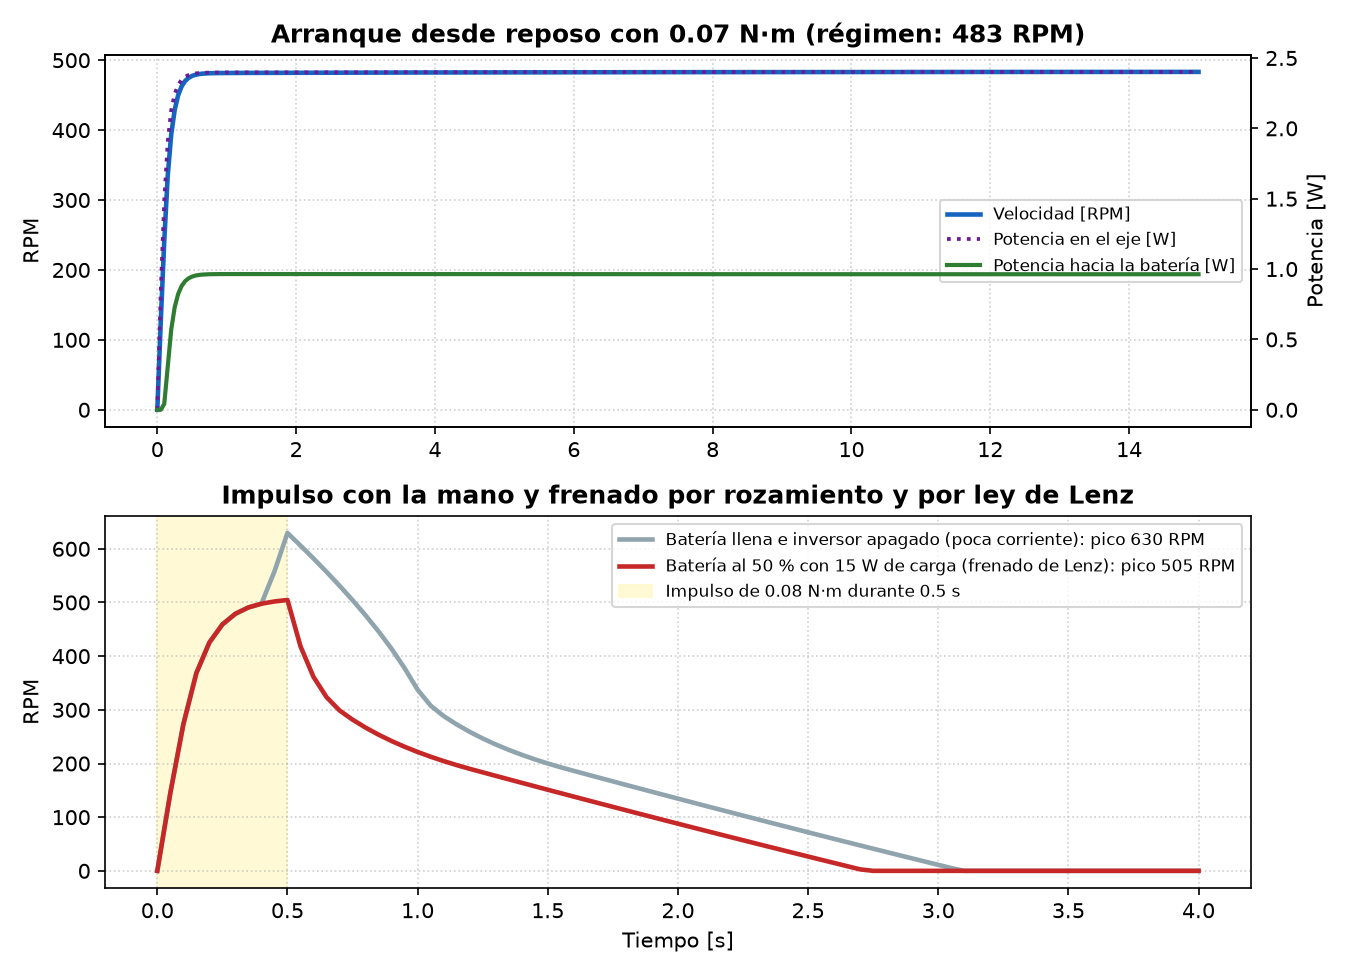
\includegraphics[width=\linewidth]{10_arranque_impulso_y_frenado.png}
      \\{\scriptsize\color{Gris}Impulso de \SI{\ValParImpulso}{N.m}: pico de \ValRpmPicoImpulso{} RPM y parada en \SI{\ValTiempoParadaImpulso}{s}.}
    \column{0.49\textwidth}
      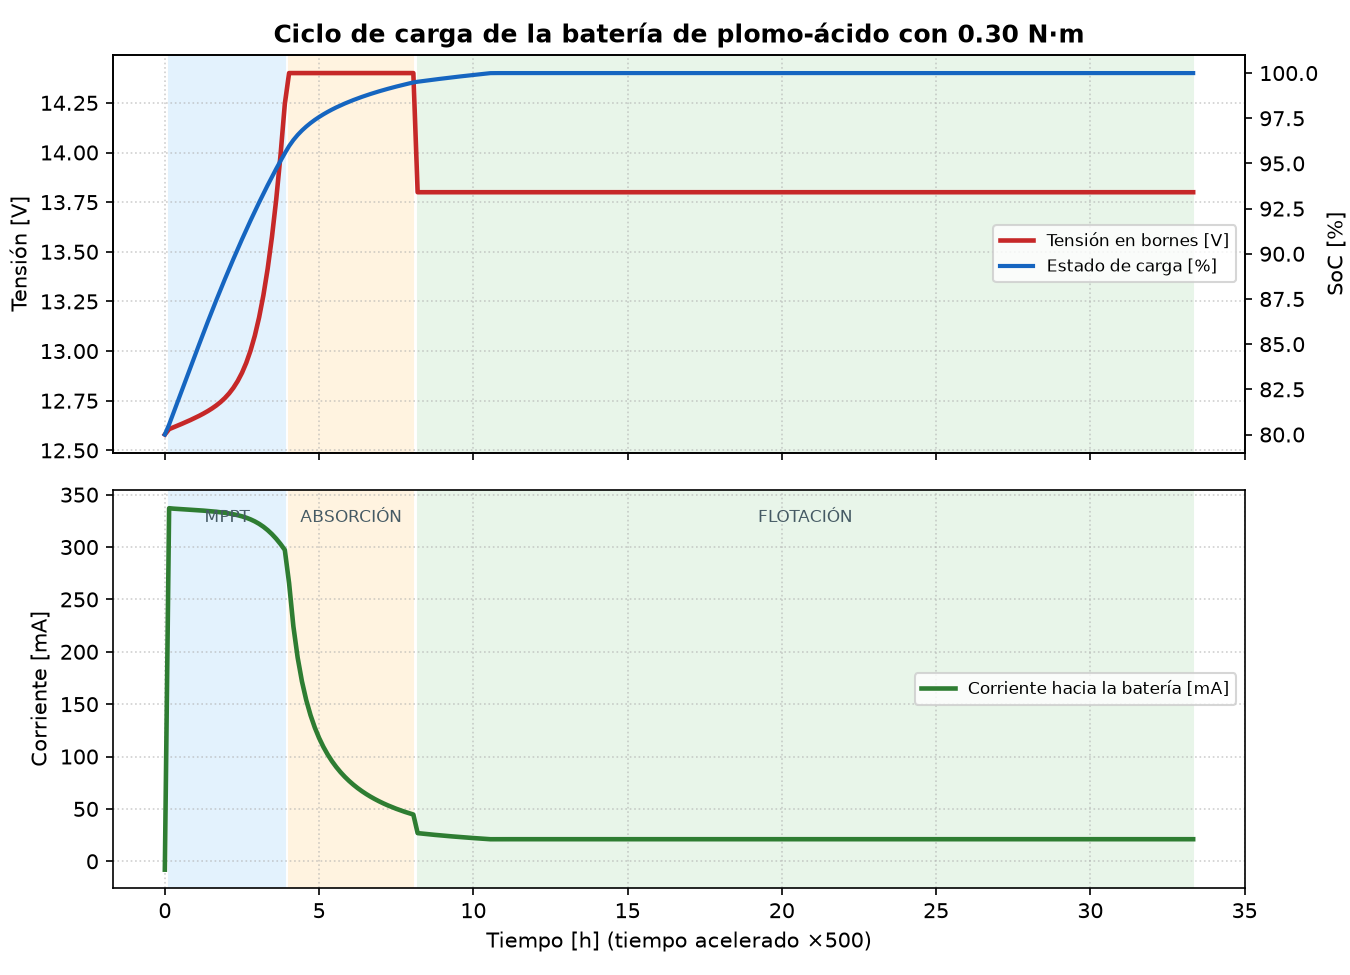
\includegraphics[width=\linewidth]{12_ciclo_de_carga_bateria.png}
      \\{\scriptsize\color{Gris}MPPT \(\to\) absorción en \SI{\ValHorasHastaAbsorcion}{h} \(\to\) flotación en \SI{\ValHorasHastaFlotacion}{h}.}
  \end{columns}
\end{frame}

% ================================================================ 7. Software  (0:30)
\begin{frame}{Arquitectura del software}
  \centering
  \begin{tikzpicture}[
      capa/.style={draw=Azul,fill=Azul!6,rounded corners=3pt,minimum height=0.8cm,
                   minimum width=2.4cm,align=center,font=\scriptsize},
      flecha/.style={-{Stealth[length=2mm]},thick,Gris},
      node distance=0.35cm]
    \node[capa] (pres) {presentación\\CLI};
    \node[capa,right=of pres] (infra) {infraestructura\\CAD, gráficas, LaTeX};
    \node[capa,right=of infra] (app) {aplicación\\simuladores};
    \node[capa,right=of app,draw=Verde,fill=Verde!8] (dom) {dominio\\física pura};
    \draw[flecha] (pres) -- (infra);
    \draw[flecha] (infra) -- (app);
    \draw[flecha] (app) -- (dom);
    \node[capa,draw=Naranja,fill=Naranja!8,minimum width=6.2cm,anchor=north]
      (js) at ([yshift=-1.0cm]$(app.south)!0.5!(dom.south)$)
      {Visualizador Three.js: \texttt{dinamica.js}, espejo exacto del modelo};
    \draw[flecha,<->,Naranja] (dom.south) -- node[right,font=\tiny,text=Naranja]
      {paridad \(10^{-9}\)} (dom.south |- js.north);
  \end{tikzpicture}

  \vspace{0.45cm}
  \begin{columns}[T]
    \column{0.23\textwidth}\centering\dato{Pruebas unitarias}{109}
    \column{0.23\textwidth}\centering\dato{Pruebas E2E}{29}
    \column{0.23\textwidth}\centering\dato{Gráficas generadas}{12}
    \column{0.23\textwidth}\centering\dato{Piezas STL}{4}
  \end{columns}
  \vspace{4pt}
  \begin{center}\scriptsize\color{Gris}
    Una única fuente de verdad (\texttt{configuracion.py}) alimenta el modelo, las piezas 3D, las gráficas y estos documentos.
  \end{center}
\end{frame}

% ================================================================ 8. Demo  (3:30)
\begin{frame}{Demostración en vivo}
  \begin{columns}[c]
    \column{0.56\textwidth}
      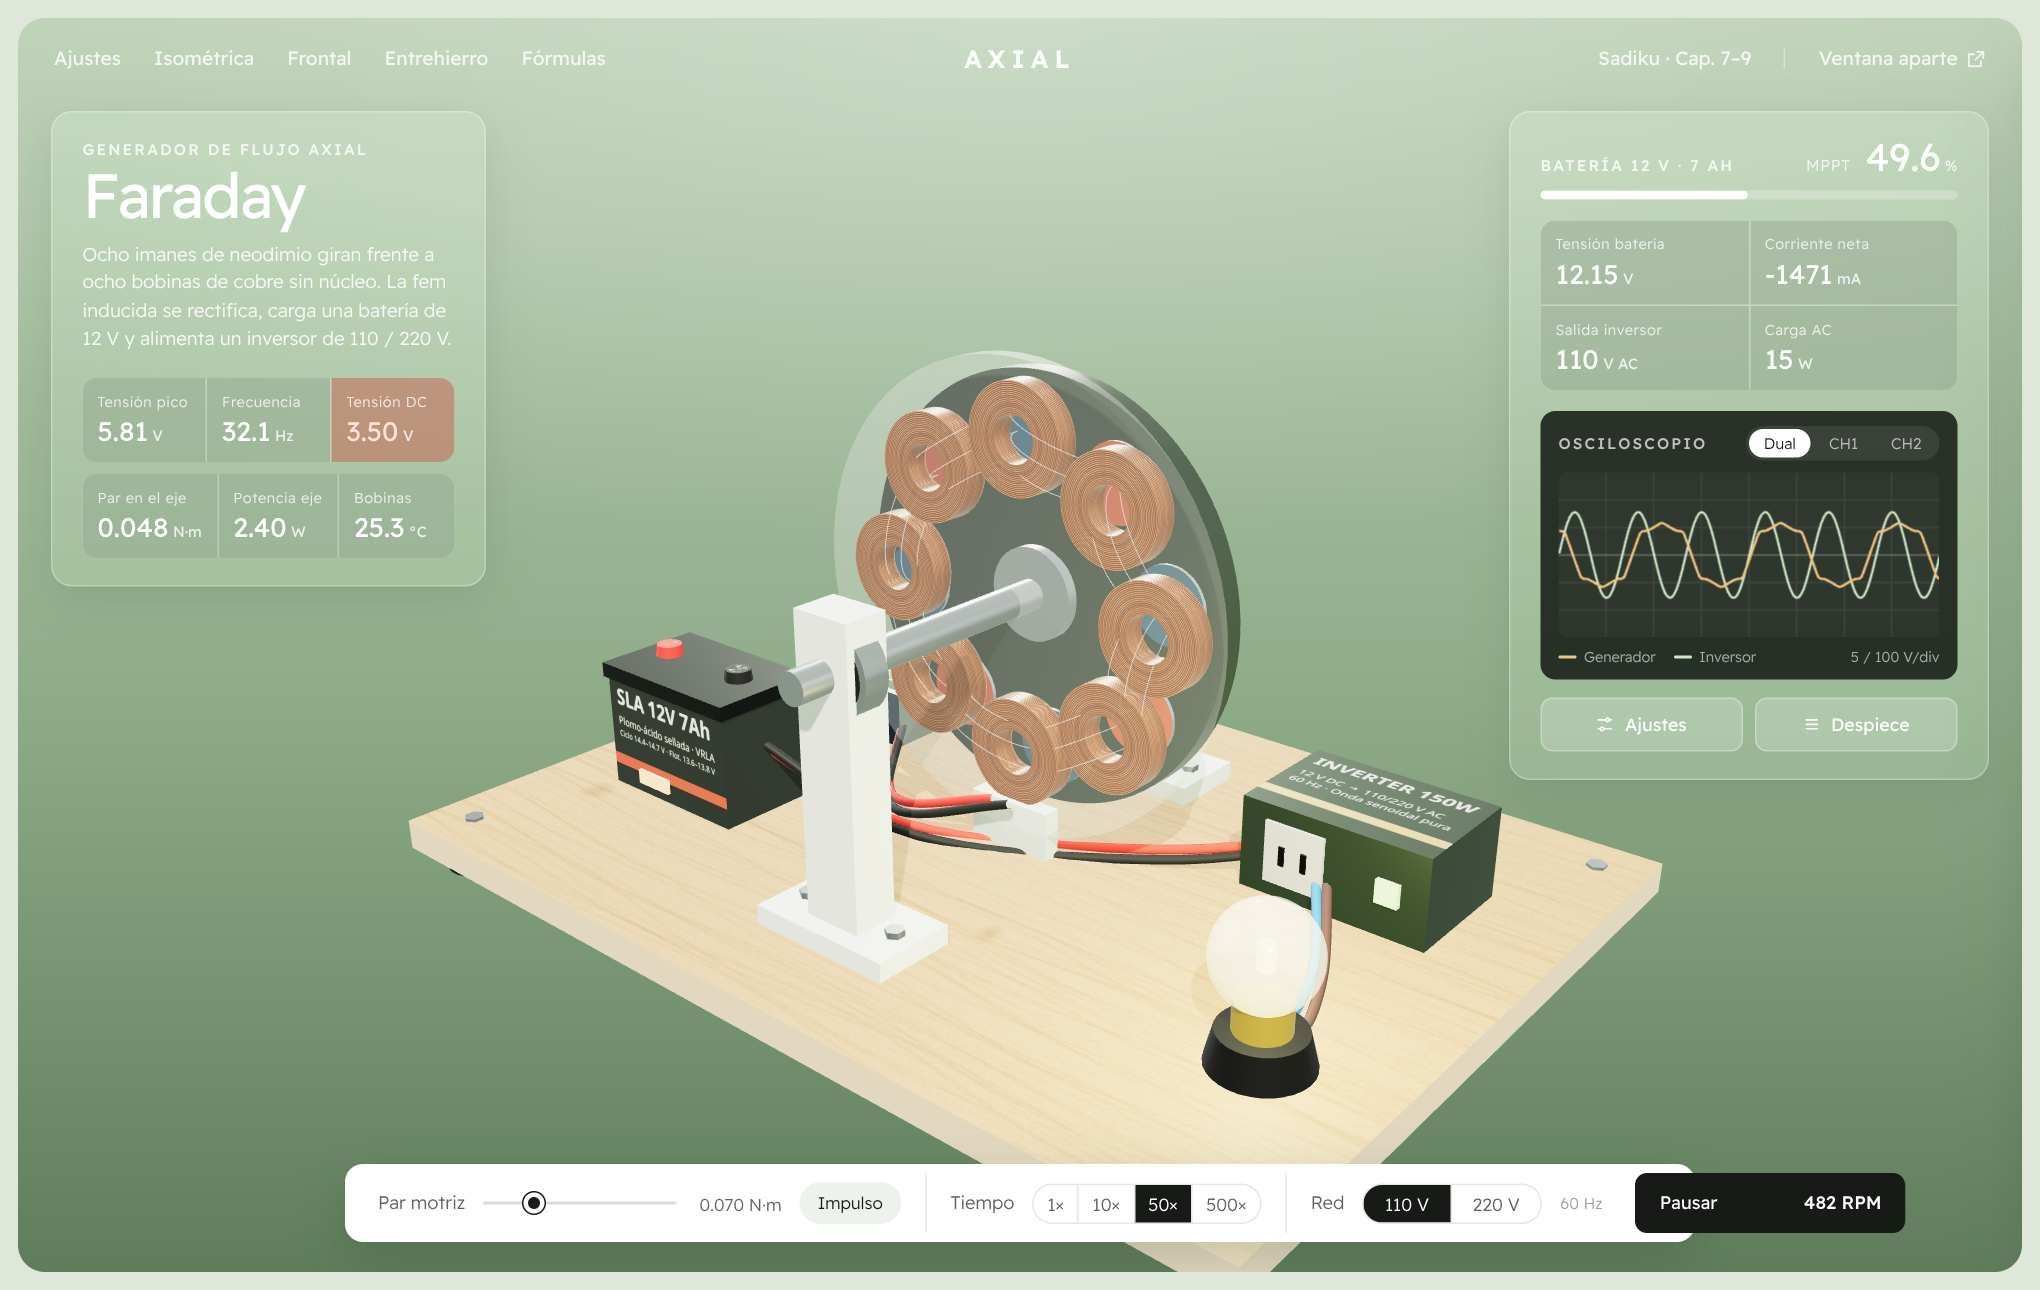
\includegraphics[width=\linewidth]{simulador_general.png}
      \\{\tiny\color{Gris}\texttt{uv run python visualizador\_3d/server.py}}
    \column{0.41\textwidth}
      \scriptsize
      \begin{enumerate}
        \setlength{\itemsep}{1pt}
        \item \textbf{Faraday}: par \SI{0.05}{N.m}, onda real en el osciloscopio.
        \item \textbf{Lenz}: par a 0 e \emph{Impulso}; el rotor frena solo.
        \item \textbf{Régimen}: par \SI{\ValParReferencia}{N.m} \(\to\) \(\approx\)\ValRpmRegimenRef{} RPM.
        \item \textbf{Micro-red}: carga \SI{15}{W}; la batería se descarga.
        \item \textbf{Carga}: inversor apagado, par \SI{\ValParMaximoMotriz}{N.m} y tiempo \(500\times\); el SoC sube.
        \item \textbf{Diseño}: entrehierro y condensador en \emph{Ajustes}.
        \item \textbf{Despiece} y cámaras.
      \end{enumerate}
  \end{columns}
\end{frame}

% ================================================================ 9. Resultados  (0:40)
\begin{frame}{Resultados del modelo realista}
  \begin{columns}[c]
    \column{0.5\textwidth}
      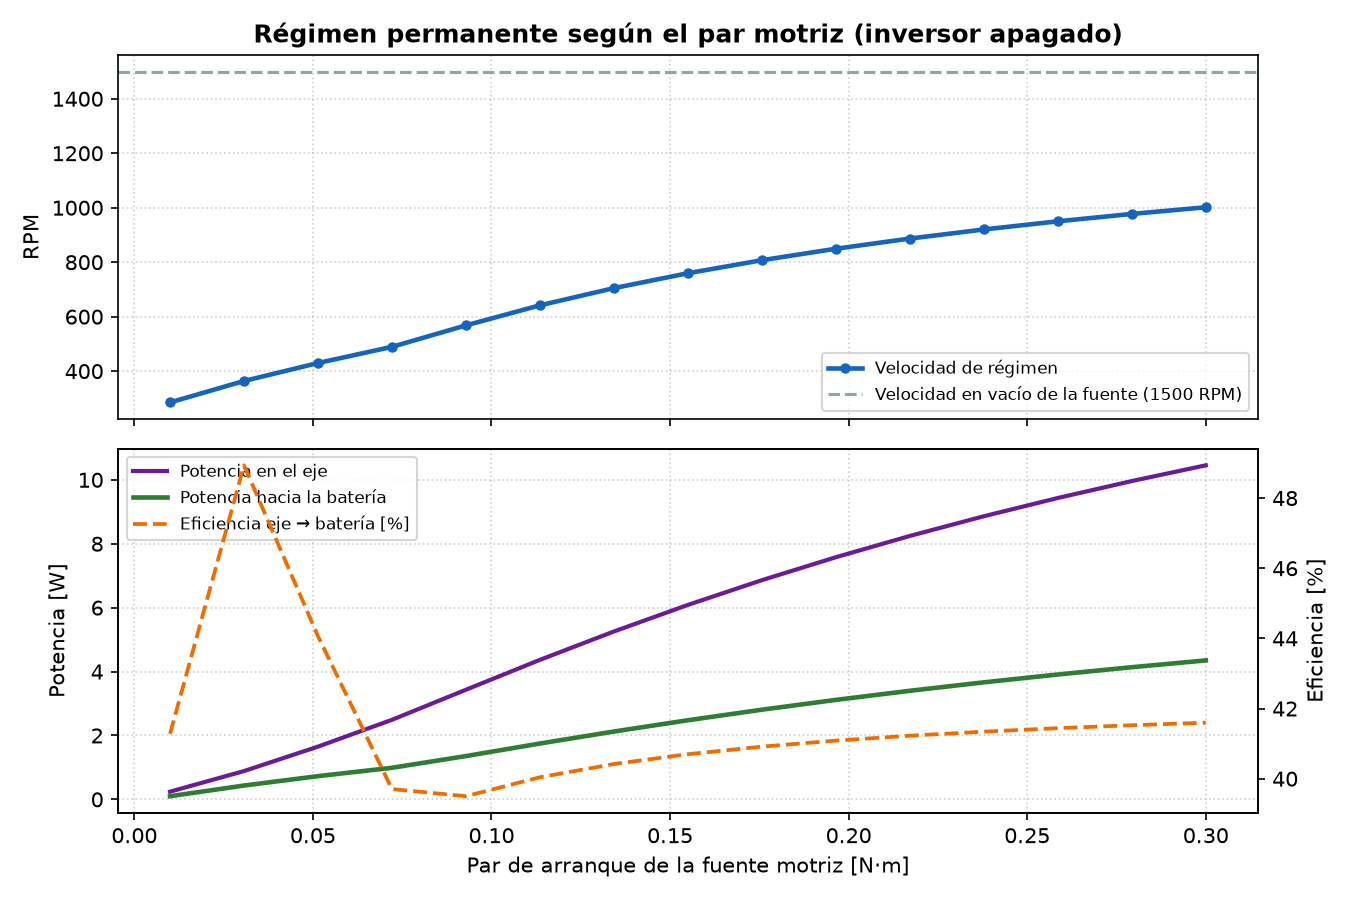
\includegraphics[width=\linewidth]{11_regimen_vs_par_motriz.png}
    \column{0.46\textwidth}
      \footnotesize
      \begin{tabular}{@{}lr@{}}
        \toprule
        \multicolumn{2}{@{}l}{\textbf{Par motriz de \SI{\ValParReferencia}{N.m}}}\\
        \midrule
        Velocidad de régimen & \ValRpmRegimenRef{} RPM\\
        Potencia en el eje & \SI{\ValPotenciaEjeRef}{W}\\
        Potencia a la batería & \SI{\ValPotenciaBateriaRef}{W}\\
        Eficiencia global & \SI{\ValEficienciaRef}{\percent}\\
        Temperatura de bobinas & \SI{\ValTemperaturaRegimenRef}{\celsius}\\
        \midrule
        \multicolumn{2}{@{}l}{\textbf{Par máximo de \SI{\ValParMaximoMotriz}{N.m}}}\\
        \midrule
        Velocidad & \ValRpmParMaximo{} RPM\\
        Potencia a la batería & \SI{\ValPotenciaBateriaParMaximo}{W}\\
        \bottomrule
      \end{tabular}
  \end{columns}
\end{frame}

% ================================================================ 10. Conclusiones  (0:20)
\begin{frame}{Conclusiones}
  \begin{columns}[T]
    \column{0.6\textwidth}
      \begin{itemize}
        \item La ley de Faraday explica la tensión generada; la ley de Lenz explica por qué cuesta girar el rotor.
        \item Sin núcleo de hierro, el generador entrega pocos vatios: sirve para cargar la batería
              despacio, no para alimentar la carga AC de forma continua.
        \item El modelo realista cambia los números: onda no senoidal, umbral del MPPT y pérdidas térmicas.
        \item El simulador reproduce el mismo modelo verificado en Python, por lo que la demo muestra resultados calculados.
      \end{itemize}
    \column{0.36\textwidth}
      \begin{alertblock}{Mejoras posibles}\small
        Más espiras o un estator doble, imanes N52 y un entrehierro menor.
      \end{alertblock}
      \vspace{0.4cm}
      \begin{center}
        {\Large\bfseries\color{Azul}¿Preguntas?}\\[4pt]
        {\tiny\color{Gris}github.com/EmanuelOrozco/axial-flux-generator}
      \end{center}
  \end{columns}
\end{frame}

\end{document}
